\documentclass[a4paper]{article}

\def\npart {IB}
\def\nterm {Lent}
\def\nyear {2016}
\def\nlecturer {P. F. Linden}
\def\ncourse {Fluid Dynamics}
\def\nlectures {TT.11}
\def\nnotready {}

% Imports
\ifx \nextra \undefined
  \usepackage[pdftex,
    hidelinks,
    pdfauthor={Dexter Chua},
    pdfsubject={Cambridge Maths Notes: Part \npart\ - \ncourse},
    pdftitle={Part \npart\ - \ncourse},
  pdfkeywords={Cambridge Mathematics Maths Math \npart\ \nterm\ \nyear\ \ncourse}]{hyperref}
  \title{Part \npart\ - \ncourse}
\else
  \usepackage[pdftex,
    hidelinks,
    pdfauthor={Dexter Chua},
    pdfsubject={Cambridge Maths Notes: Part \npart\ - \ncourse\ (\nextra)},
    pdftitle={Part \npart\ - \ncourse\ (\nextra)},
  pdfkeywords={Cambridge Mathematics Maths Math \npart\ \nterm\ \nyear\ \ncourse\ \nextra}]{hyperref}

  \title{Part \npart\ - \ncourse \\ {\Large \nextra}}
\fi

\author{Lectured by \nlecturer \\\small Notes taken by Dexter Chua}
\date{\nterm\ \nyear}

\usepackage{alltt}
\usepackage{amsfonts}
\usepackage{amsmath}
\usepackage{amssymb}
\usepackage{amsthm}
\usepackage{booktabs}
\usepackage{caption}
\usepackage{enumitem}
\usepackage{fancyhdr}
\usepackage{graphicx}
\usepackage{mathtools}
\usepackage{microtype}
\usepackage{multirow}
\usepackage{pdflscape}
\usepackage{pgfplots}
\usepackage{siunitx}
\usepackage{tabularx}
\usepackage{tikz}
\usepackage{tkz-euclide}
\usepackage[normalem]{ulem}
\usepackage[all]{xy}

\pgfplotsset{compat=1.12}

\pagestyle{fancyplain}
\lhead{\emph{\nouppercase{\leftmark}}}
\ifx \nextra \undefined
  \rhead{
    \ifnum\thepage=1
    \else
      \npart\ \ncourse
    \fi}
\else
  \rhead{
    \ifnum\thepage=1
    \else
      \npart\ \ncourse\ (\nextra)
    \fi}
\fi
\usetikzlibrary{arrows}
\usetikzlibrary{decorations.markings}
\usetikzlibrary{decorations.pathmorphing}
\usetikzlibrary{positioning}
\usetikzlibrary{fadings}
\usetikzlibrary{intersections}
\usetikzlibrary{cd}

\newcommand*{\Cdot}{\raisebox{-0.25ex}{\scalebox{1.5}{$\cdot$}}}
\newcommand {\pd}[2][ ]{
  \ifx #1 { }
    \frac{\partial}{\partial #2}
  \else
    \frac{\partial^{#1}}{\partial #2^{#1}}
  \fi
}

% Theorems
\theoremstyle{definition}
\newtheorem*{aim}{Aim}
\newtheorem*{axiom}{Axiom}
\newtheorem*{claim}{Claim}
\newtheorem*{cor}{Corollary}
\newtheorem*{defi}{Definition}
\newtheorem*{eg}{Example}
\newtheorem*{fact}{Fact}
\newtheorem*{law}{Law}
\newtheorem*{lemma}{Lemma}
\newtheorem*{notation}{Notation}
\newtheorem*{prop}{Proposition}
\newtheorem*{thm}{Theorem}

\renewcommand{\labelitemi}{--}
\renewcommand{\labelitemii}{$\circ$}
\renewcommand{\labelenumi}{(\roman{*})}

\let\stdsection\section
\renewcommand\section{\newpage\stdsection}

% Strike through
\def\st{\bgroup \ULdepth=-.55ex \ULset}

% Maths symbols
\newcommand{\bra}{\langle}
\newcommand{\ket}{\rangle}

\newcommand{\N}{\mathbb{N}}
\newcommand{\Z}{\mathbb{Z}}
\newcommand{\Q}{\mathbb{Q}}
\renewcommand{\H}{\mathbb{H}}
\newcommand{\R}{\mathbb{R}}
\newcommand{\C}{\mathbb{C}}
\newcommand{\Prob}{\mathbb{P}}
\renewcommand{\P}{\mathbb{P}}
\newcommand{\E}{\mathbb{E}}
\newcommand{\F}{\mathbb{F}}
\newcommand{\cU}{\mathcal{U}}
\newcommand{\RP}{\mathbb{RP}}
\newcommand{\CP}{\mathbb{CP}}

\newcommand{\ph}{\,\cdot\,}

\DeclareMathOperator{\sech}{sech}
\DeclareMathOperator{\cosech}{cosech}
\DeclareMathOperator{\cosec}{cosec}

\DeclareMathOperator{\covol}{covol}
\DeclareMathOperator{\vol}{vol}

\let\Im\relax
\let\Re\relax
\DeclareMathOperator{\Im}{Im}
\DeclareMathOperator{\Re}{Re}
\DeclareMathOperator{\im}{im}
\DeclareMathOperator{\image}{image}
\DeclareMathOperator{\Ann}{Ann}

\DeclareMathOperator*{\res}{res}
\DeclareMathOperator{\Res}{Res}
\DeclareMathOperator{\Ind}{Ind}

\DeclareMathOperator{\tr}{tr}
\DeclareMathOperator{\diag}{diag}
\DeclareMathOperator{\rank}{rank}
\DeclareMathOperator{\card}{card}
\DeclareMathOperator{\spn}{span}
\DeclareMathOperator{\adj}{adj}

\DeclareMathOperator{\erf}{erf}
\DeclareMathOperator{\erfc}{erfc}

\DeclareMathOperator{\ord}{ord}
\DeclareMathOperator{\Sym}{Sym}

\DeclareMathOperator{\sgn}{sgn}
\DeclareMathOperator{\orb}{orb}
\DeclareMathOperator{\stab}{stab}
\DeclareMathOperator{\ccl}{ccl}

\DeclareMathOperator{\lcm}{lcm}
\DeclareMathOperator{\hcf}{hcf}

\DeclareMathOperator{\Int}{Int}
\DeclareMathOperator{\id}{id}

\DeclareMathOperator{\betaD}{beta}
\DeclareMathOperator{\gammaD}{gamma}
\DeclareMathOperator{\Poisson}{Poisson}
\DeclareMathOperator{\binomial}{binomial}
\DeclareMathOperator{\multinomial}{multinomial}
\DeclareMathOperator{\Bernoulli}{Bernoulli}
\DeclareMathOperator{\like}{like}

\DeclareMathOperator{\var}{var}
\DeclareMathOperator{\cov}{cov}
\DeclareMathOperator{\bias}{bias}
\DeclareMathOperator{\mse}{mse}
\DeclareMathOperator{\corr}{corr}

\DeclareMathOperator{\otp}{otp}
\DeclareMathOperator{\dom}{dom}

\DeclareMathOperator{\Root}{Root}
\DeclareMathOperator{\supp}{supp}
\DeclareMathOperator{\rel}{rel}
\DeclareMathOperator{\Hom}{Hom}
\DeclareMathOperator{\Aut}{Aut}
\DeclareMathOperator{\Gal}{Gal}
\DeclareMathOperator{\Mat}{Mat}
\DeclareMathOperator{\End}{End}
\DeclareMathOperator{\Char}{char}
\DeclareMathOperator{\ev}{ev}
\DeclareMathOperator{\St}{St}
\DeclareMathOperator{\Lk}{Lk}
\DeclareMathOperator{\disc}{disc}
\DeclareMathOperator{\Isom}{Isom}
\DeclareMathOperator{\length}{length}
\DeclareMathOperator{\energy}{energy}
\DeclareMathOperator{\area}{area}
\DeclareMathOperator{\Syl}{Syl}
\DeclareMathOperator{\cl}{cl}
\DeclareMathOperator{\fix}{fix}

\newcommand{\GL}{\mathrm{GL}}
\newcommand{\SL}{\mathrm{SL}}
\newcommand{\PGL}{\mathrm{PGL}}
\newcommand{\PSL}{\mathrm{PSL}}
\newcommand{\PSU}{\mathrm{PSU}}
\newcommand{\Or}{\mathrm{O}}
\newcommand{\SO}{\mathrm{SO}}
\newcommand{\U}{\mathrm{U}}
\newcommand{\SU}{\mathrm{SU}}

\renewcommand{\d}{\mathrm{d}}
\newcommand{\D}{\mathrm{D}}

\tikzset{->/.style = {decoration={markings,
                                  mark=at position 1 with {\arrow[scale=2]{latex'}}},
                      postaction={decorate}}}
\tikzset{<-/.style = {decoration={markings,
                                  mark=at position 0 with {\arrowreversed[scale=2]{latex'}}},
                      postaction={decorate}}}
\tikzset{<->/.style = {decoration={markings,
                                   mark=at position 0 with {\arrowreversed[scale=2]{latex'}},
                                   mark=at position 1 with {\arrow[scale=2]{latex'}}},
                       postaction={decorate}}}
\tikzset{->-/.style = {decoration={markings,
                                   mark=at position #1 with {\arrow[scale=2]{latex'}}},
                       postaction={decorate}}}
\tikzset{-<-/.style = {decoration={markings,
                                   mark=at position #1 with {\arrowreversed[scale=2]{latex'}}},
                       postaction={decorate}}}

\tikzset{circ/.style = {fill, circle, inner sep = 0, minimum size = 3}}
\tikzset{mstate/.style={circle, draw, blue, text=black, minimum width=0.7cm}}

\definecolor{mblue}{rgb}{0.2, 0.3, 0.8}
\definecolor{morange}{rgb}{1, 0.5, 0}
\definecolor{mgreen}{rgb}{0.1, 0.4, 0.2}
\definecolor{mred}{rgb}{0.5, 0, 0}

\def\drawcirculararc(#1,#2)(#3,#4)(#5,#6){%
    \pgfmathsetmacro\cA{(#1*#1+#2*#2-#3*#3-#4*#4)/2}%
    \pgfmathsetmacro\cB{(#1*#1+#2*#2-#5*#5-#6*#6)/2}%
    \pgfmathsetmacro\cy{(\cB*(#1-#3)-\cA*(#1-#5))/%
                        ((#2-#6)*(#1-#3)-(#2-#4)*(#1-#5))}%
    \pgfmathsetmacro\cx{(\cA-\cy*(#2-#4))/(#1-#3)}%
    \pgfmathsetmacro\cr{sqrt((#1-\cx)*(#1-\cx)+(#2-\cy)*(#2-\cy))}%
    \pgfmathsetmacro\cA{atan2(#2-\cy,#1-\cx)}%
    \pgfmathsetmacro\cB{atan2(#6-\cy,#5-\cx)}%
    \pgfmathparse{\cB<\cA}%
    \ifnum\pgfmathresult=1
        \pgfmathsetmacro\cB{\cB+360}%
    \fi
    \draw (#1,#2) arc (\cA:\cB:\cr);%
}
\newcommand\getCoord[3]{\newdimen{#1}\newdimen{#2}\pgfextractx{#1}{\pgfpointanchor{#3}{center}}\pgfextracty{#2}{\pgfpointanchor{#3}{center}}}

\def\Xint#1{\mathchoice
   {\XXint\displaystyle\textstyle{#1}}%
   {\XXint\textstyle\scriptstyle{#1}}%
   {\XXint\scriptstyle\scriptscriptstyle{#1}}%
   {\XXint\scriptscriptstyle\scriptscriptstyle{#1}}%
   \!\int}
\def\XXint#1#2#3{{\setbox0=\hbox{$#1{#2#3}{\int}$}
     \vcenter{\hbox{$#2#3$}}\kern-.5\wd0}}
\def\ddashint{\Xint=}
\def\dashint{\Xint-}


\begin{document}
\maketitle
{\small
\noindent\textbf{Parallel viscous flow}\\
Plane Couette flow, dynamic viscosity. Momentum equation and boundary conditions. Steady flows including Poiseuille flow in a channel. Unsteady flows, kinematic viscosity, brief description of viscous boundary layers (skin depth).\hspace*{\fill} [3]

\vspace{10pt}
\noindent\textbf{Kinematics}\\
Material time derivative. Conservation of mass and the kinematic boundary condition. Incompressibility; streamfunction for two-dimensional flow. Streamlines and path lines.\hspace*{\fill} [2]

\vspace{10pt}
\noindent\textbf{Dynamics}\\
Statement of Navier-Stokes momentum equation. Reynolds number. Stagnation-point flow; discussion of viscous boundary layer and pressure field. Conservation of momentum; Euler momentum equation. Bernoulli's equation.

\vspace{5pt}
\noindent Vorticity, vorticity equation, vortex line stretching, irrotational flow remains irrotational. \hspace*{\fill} [4]

\vspace{10pt}
\noindent\textbf{Potential flows}\\
Velocity potential; Laplace's equation, examples of solutions in spherical and cylindrical geometry by separation of variables. Translating sphere. Lift on a cylinder with circulation.

\vspace{5pt}
\noindent Expression for pressure in time-dependent potential flows with potential forces. Oscillations in a manometer and of a bubble.\hspace*{\fill} [3]

\vspace{10pt}
\noindent\textbf{Geophysical flows}\\
Linear water waves: dispersion relation, deep and shallow water, standing waves in a container, Rayleigh-Taylor instability.

\vspace{5pt}
\noindent Euler equations in a rotating frame. Steady geostrophic flow, pressure as streamfunction. Motion in a shallow layer, hydrostatic assumption, modified continuity equation. Conservation of potential vorticity, Rossby radius of deformation.\hspace*{\fill} [4]}

\tableofcontents
\setcounter{section}{-1}
\section{Introduction}
In real life, we encounter a lot of fluids. For example, there is air and water. These are known as \emph{Newtonian fluids}, whose dynamics follow relatively simple equations. This is fundamentally because they have simple composition --- they are made up of simple molecules. An example of \emph{non-Newtonian} fluid is shampoo, which, despite looking innocent, has long chain molecules with complex properties.

In fluid dynamics, one of the most important things is to distinguish what is a fluid and what is not. For example, air and water are fluids, while the wall is solid. A main distinction is that we can lean on the wall, but not on air and water. In particular, if we apply a force on the wall, it will deform a bit, but then stop. A finite force on a solid will lead to a finite deformation. On the other hand, if we attempt to apply a force onto air or water, it will just move along the direction of force indefinitely. A finite force can lead to infinite deformation.

This is the main difference between solid mechanics and fluid mechanics. In solid mechanics, we look at properties like elasticity. This measures how much deformation we get when we apply a force. In fluid mechanics, we don't measure distances, since they can potentially be infinite. Instead, we would often be interested in the velocity of fluids.

There are many applications of fluid dynamics. On a small scale, the dynamics of fluids in cells is important for biology. On a larger scale, the fluid flow of the mantle affects the movement of tectonic plates, while the dynamics of the atmosphere can be used to explain climate and weather. On an even larger scale, we can use fluid dynamics to analyse the flow of galactic systems in the universe.

\section{Parallel viscous flow}
\setcounter{subsection}{-1}
\subsection{Preliminaries}
This section is called preliminaries, not definitions, because the ``definitions'' we give will be a bit fuzzy. We will (hopefully) get better definitions later on.

\begin{defi}[Fluid]
  A \emph{fluid} is a material that flows.
\end{defi}

\begin{eg}
  Air, water and oil are fluids. These are known as \emph{simple} or \emph{Newtonian} fluids, because they are simple.

  Paint, toothpaste and shampoo are \emph{complex} or \emph{non-Newtonian} fluids, because they are complicated.

  Sand, rice and foams are \emph{granular flows}. These have some fluid-like properties, but are fundamentally made of small granular solids.
\end{eg}

In this course, we will restrict our attention to Newtonian fluids, with a technical definition given as follows:

\begin{defi}[Newtonian fluids and viscosity]
  A \emph{Newtonian fluid} is a fluid with a linear relationship between stress and rate of strain. The constant of proportionality is \emph{viscosity}.
\end{defi}
We will soon define what these words mean, but the key point is linearity.

\begin{defi}[Stress]
  \emph{Stress} is force per unit area.
\end{defi}
For example, pressure is a stress.

\begin{defi}[Strain]
  \emph{Strain} is the extension per unit length. The \emph{rate of strain} is $\frac{\d}{\d t}(\mathrm{strain})$ is concerned with gradients of velocity.
\end{defi}
These quantities are in fact tensor fields, but we will not treat them as such in this course. We will just consider ``simplified'' cases. For the full-blown treatment with tensor fields, refer to the Part II course.

While all fluids are viscous, much of the course will use the \emph{inviscid approximation}, ie. we set the viscosity to be $0$.

We will first consider the special case, where the flow moves along parallel planes.

\subsection{Stress}
\subsubsection{Normal stress}
\begin{center}
  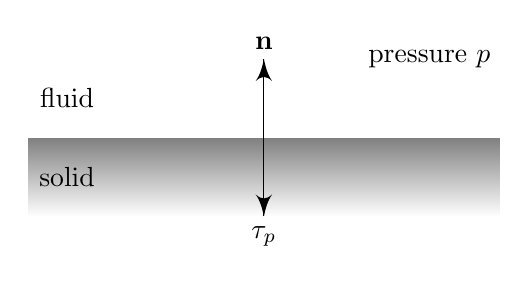
\begin{tikzpicture}
    \fill [gray, path fading=south] (0, 0) rectangle (6, -1);
    \draw [->] (3, 0) -- +(0, 1) node [above] {$\mathbf{n}$};
    \draw [->] (3, 0) -- +(0, -1) node [below] {$\tau_p$};
    \node at (0.5, -0.5) {solid};
    \node at (0.5, 0.5) {fluid};
    \node at (6, 1) [left] {pressure $p$};
  \end{tikzpicture}
\end{center}
Suppose we have a fluid with pressure $p$ acting on a surface with unit normal $\mathbf{n}$, pointing \emph{into} the fluid.

\begin{defi}[Normal stress]
  The \emph{normal stress} is
  \[
    \tau_p = -p\mathbf{n}.
  \]
\end{defi}
Gradients in pressure produce a force. For example, suppose we have a pipe, with the pump on the left:
\begin{center}
  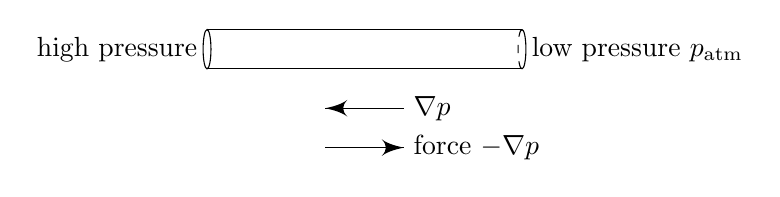
\begin{tikzpicture}
    \draw (0, 0) -- +(4, 0);
    \node at (0, 0.25) [left] {high pressure};
    \node at (4, 0.25) [right] {low pressure $p_{\mathrm{atm}}$};
    \draw (0, 0.5) -- +(4, 0);
    \draw [->] (2.5, -0.5) node [right] {$\nabla p$} -- +(-1, 0);
    \draw [->] (1.5, -1) -- +(1, 0) node [right] {force $-\nabla p$};
    \draw (0, 0.25) ellipse (0.05 and 0.25);
    \draw [dashed] (4, 0) arc (270:90:0.05 and 0.25);
    \draw (4, 0) arc (270:450:0.05 and 0.25);
  \end{tikzpicture}
\end{center}
This gives a \emph{body force} that drives the water from left to right.

\subsubsection{Tangential stress}
Consider two infinite planes with fluids in between. We keep the bottom plane at rest, and move the top plate with velocity $U$.
\begin{center}
  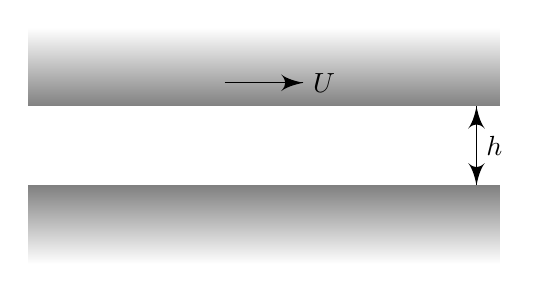
\begin{tikzpicture}
    \fill [gray, path fading=south] (0, 0) rectangle (6, -1);
    \fill [gray, path fading=north] (0, 1) rectangle (6, 2);
    \draw [->] (2.5, 1.3) -- +(1, 0) node [right] {$U$};

    \draw [<->] (5.7, 0) -- +(0, 1) node [right, pos=0.5] {$h$};
  \end{tikzpicture}
\end{center}

\begin{defi}[Tangential stress]
  The \emph{tangential stress} $\tau_s$ is the force (per unit area) required to move the top plate at speed $U$.
\end{defi}

Experimentally, we find the following.
\begin{law}
  For a Newtonian fluid, we have
  \[
    \tau_s \propto \frac{U}{h}.
  \]
\end{law}

\begin{defi}[Dynamic viscosity]
  The \emph{dynamic viscosity} $\mu$ of the fluid is the constant of proportionality in
  \[
    \tau_s = \mu \frac{U}{h}.
  \]
\end{defi}

We find the dimensions of these quantities as
\begin{align*}
  [\tau_s] &= ML^{-1} T^{-2}\\
  \left[\frac{U}{h}\right] &= T^{-1}\\
  [\mu] &= ML^{-1} T^{-1}.
\end{align*}
In SI units, $\mu$ has units $\SI{}{\kilo\gram\per\meter\per\second}$.

We have not yet said what the fluid in the middle does. It turns out this is simple: at the bottom, the fluid is constant, and at the top, the fluid moves with velocity $U$. In between, the speed varies linearly.
\begin{center} % put axes in gray
  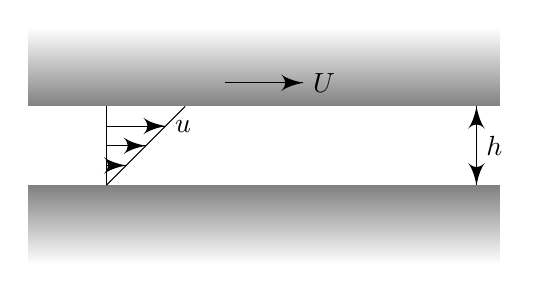
\begin{tikzpicture}
    \fill [gray, path fading=south] (0, 0) rectangle (6, -1);
    \fill [gray, path fading=north] (0, 1) rectangle (6, 2);
    \draw [->] (2.5, 1.3) -- +(1, 0) node [right] {$U$};

    \draw [<->] (5.7, 0) -- +(0, 1) node [right, pos=0.5] {$h$};

    \draw (1, 0) -- (1, 1);
    \draw (1, 0) -- (2, 1);
    \foreach \x in {0,0.25,0.5,0.75} {
      \draw [->] (1, \x) -- (1 + \x, \x);
    }
    \node at (1.75, 0.75) [right] {$u$};
  \end{tikzpicture}
\end{center}
We will derive this formally later.

For a general flow, let $u_T(\mathbf{x})$ be the velocity of the fluid at position $\mathbf{x}$. Then the tangential stress is
\[
  \tau_s = \mu \frac{\partial u_T(\mathbf{x})}{\partial \mathbf{n}},
\]
and is in the direction of the tangential component of velocity. Again, the normal vector $\mathbf{n}$ points \emph{into} the fluid.

\subsection{Steady parallel viscous flow}
We first explain what the words in the title mean. Steady means there is no change in time, ie. there is no acceleration. In other words, all forces balance.

``Parallel'' means the fluid only flows in one dimension, and only depends on the direction perpendicular to the plane. So the velocity can be written as
\[
  \mathbf{u} = (u(y), 0, 0).
\]
We can draw a flow profile as follows:
\begin{center}
  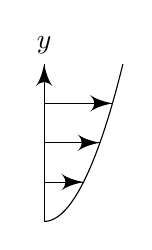
\begin{tikzpicture}
    \draw (0, 0) parabola (1, 2);
    \foreach \x in {0,0.25,0.5,0.75} {
      \pgfmathsetmacro\len{sqrt(\x)}
      \draw [->] (0, 2*\x) -- +(\len, 0);
    }
    \draw [->] (0, 0) -- (0, 2) node [above] {$y$};
  \end{tikzpicture}
\end{center}
We consider a small box in the fluid:
\begin{center}
  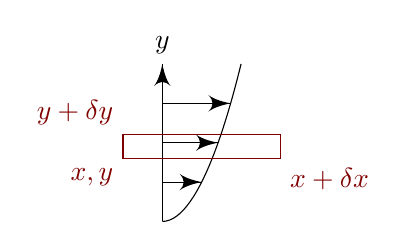
\begin{tikzpicture}
    \draw (0, 0) parabola (1, 2);
    \foreach \x in {0,0.25,0.5,0.75} {
      \pgfmathsetmacro\len{sqrt(\x)}
      \draw [->] (0, 2*\x) -- +(\len, 0);
    }
    \draw [->] (0, 0) -- (0, 2) node [above] {$y$};
    \draw [mred] (-0.5, 0.8) node [anchor = north east] {$x, y$} -- +(2, 0) node [anchor = north west] {$x + \delta x$} -- +(2, 0.3) -- +(0, 0.3) node [anchor = south east] {$y + \delta y$} -- cycle;
  \end{tikzpicture}
\end{center}
We know that this block of fluid moves in the $x$ direction without acceleration. So the total forces of the surrounding environment on the box should vanish.

We first consider the $x$ direction. There are normal stresses at the sides, and tangential stresses at the top and bottom. The sum of forces in the $x$-direction (per unit transverse width) gives
\[
  p(x) \delta y - p(x + \delta x) \delta y + \tau_s(t + \delta y) \delta x + \tau_s(\tau) \delta x = 0.
\]
By the definition of $\tau_s$, we can write
\[
  \tau_s(y + \delta y) = \mu \frac{\partial u}{\partial y}(y + \delta y),\quad \tau_s (y) = -\mu \frac{\partial u}{\partial y}(y),
\]
where the different signs come from the different normals (for a normal pointing downwards, $\frac{\partial}{\partial \mathbf{n}} = \frac{\partial}{\partial -y}$).

Dividing by $\delta x \delta y$ and take the limit as $\delta x, \delta y \to 0$, we end up with the equation of motion
\[
  -\frac{\partial p}{\partial x} + \mu \frac{\partial^2 u}{\partial y^2} = 0.\tag{1.2a}
\]
Looking at the $y$ direction, we find
\[
  -\frac{\partial p}{\partial y} = 0.\tag{1.2b}
\]
In the second equation, we keep the negative sign for consistency, but obviously in this case it is not necessary.

This is the simplest possible case. We can extend this a bit by allowing, say, non-steady flows, For unsteady parallel viscous flows
\[
  \mathbf{u} = (U(u, t), 0, 0)
\]
of an (incompressible) fluid acted on by a body force (per unit volume) $(f_x, f_y, 0)$, we obtain the equations
\begin{align*}
  \rho\frac{\partial u}{\partial t} &= -\frac{\partial p}{\partial x} + \mu \frac{\partial^2 u}{\partial y^2} + f_x\tag{1.3a}\\
  0 &=-\frac{\partial p}{\partial y} + f_y.\tag{1.3b}
\end{align*}
You will derive these in example sheet 1. Here $\rho$ is the density, ie. the mass per unit volume. For air, it is approximately $\SI{1}{\kilo\gram\per\meter\cubed}$, and for water, it is approximately $\SI{1000}{\kilo\gram\per\meter\cubed}$.

Here we said that the fluid is incompressible, which means it cannot be compressed (duh). We will give a form definition later. In general, though, fluids are not compressible. For example, sound waves are exactly waves of compression in air, and cannot exist if air is incompressible. Alternatively, we say that sound travels at an infinite speed.

Hence, compressibility matters mostly when we are travelling near the speed of sound. If we are moving in low speeds, we can just pretend the fluid is indeed incompressible.

\subsection{Boundary conditions for viscous fluids}
Experimentally, we found (down to 2 molecular diameters for water, approximately $\SI{6}{\angstrom}$) that Newtonian fluids satisfy one of the following two boundary conditions:
\begin{enumerate}
  \item \emph{No-slip condition}: at the boundary, the tangential component of the fluid velocity equals the tangential velocity of boundary. In particular, if the boundary is stable, the tangential component of the fluid velocity is zero. This means fluids stick to surfaces.
    \[
      u_T = 0.\tag{1.5}
    \]
  \item \emph{Stress condition}: alternatively, a tangential stress $\tau$ is imposed on the fluid. In this case,
    \[
      -\mu \frac{\partial u_T}{\partial n} = \tau.\tag{1.5}
    \]
\end{enumerate}

We are going to look at some examples.
\subsection{Couette flow}
This is the flow driven by the motion of a boundary.
\begin{center}
  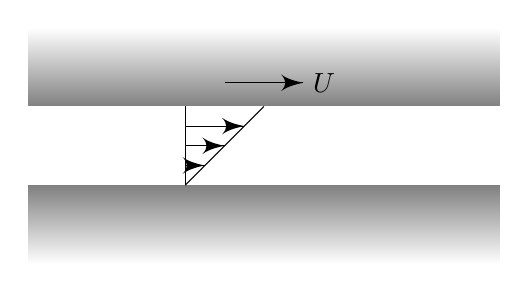
\begin{tikzpicture}
    \fill [gray, path fading=south] (0, 0) rectangle (6, -1);
    \fill [gray, path fading=north] (0, 1) rectangle (6, 2);
    \draw [->] (2.5, 1.3) -- +(1, 0) node [right] {$U$};

    \draw (2, 0) -- (2, 1);
    \draw (2, 0) -- (3, 1);

    \foreach \x in {0.25,0.5,0.75} {
      \draw [->] (2, \x) -- +(\x, 0);
    }
  \end{tikzpicture}
\end{center}
We assume that this is a stead flow, and there is no pressure gradient. So our equations give
\[
  \frac{\partial^2 u}{\partial y^2} = 0.
\]
Moreover, we have the boundary condition of $u = 0$ on $y = 0$; $u = U$ on $y = h$. The solution is thus
\[
  u = \frac{U y}{h}.
\]
\subsection{Pouseuille flow}
This is a flow driven by a pressure gradient between stationary boundaries. Again we have two boundaries
\begin{center}
  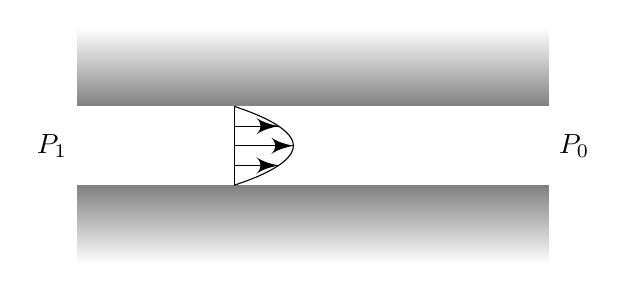
\begin{tikzpicture}
    \fill [gray, path fading=south] (0, 0) rectangle (6, -1);
    \fill [gray, path fading=north] (0, 1) rectangle (6, 2);

    \node [left] at (0, 0.5) {$P_1$};
    \node [right] at (6, 0.5) {$P_0$};

    \foreach \x in {0.25,0.5,0.75} {
      \pgfmathsetmacro\len{\x * (1 - \x)}
      \draw [->] (2, \x) -- +(3 * \len, 0);
    };
    \draw [rotate=270, yscale=-1, shift={(-3,-3)}] (2.5, 0.25) parabola (2, 1); % magic
    \draw [rotate=90, shift={(-2,-3)}] (2.5, 0.25) parabola (2, 1);
    \draw (2, 0) -- (2, 1);
  \end{tikzpicture}
\end{center}
We have a high pressure $P_1$ on the left, and a low pressure $P_0 < P_1$ on the right. We solve this problem again, but we will also include gravity. So the equations of motion become
\begin{align*}
  -\frac{\partial p}{\partial x} + \mu\frac{\partial^2 u}{\partial y^2} &= 0\\
  -\frac{\partial p}{\partial y} - g\rho &= 0
\end{align*}
The boundary conditions are $u = 0$ at $y = 0, h$. The second equation implies
\[
  p =- g\rho y + f(x)
\]
for some function $f$. Substituting into the first gives
\[
  \mu\frac{\partial^2 u}{\partial y^2} = f'(x).
\]
The left is a function of $y$ only, while the right depends only on $x$. So both must be constant, say $G$. Using the boundary conditions, we get
\[
  \mu\frac{\partial^2 u}{\partial y^2} = f'(x) = G = \frac{P_1 - P_0}{L},
\]
where $L$ is the length of the tube. Then we find
\[
  u = \frac{G}{2 \mu} y(h - y).
\]
Here the velocity is the greatest at the middle, where $y = \frac{h}{2}$.

Since the equations of motion are linear, if we have both a moving boundary and a pressure gradient, we can just add the tow solutions up.

\subsection{Derived properties of a flow}
We're going to look at some properties of these flows. One thing we want to know is how much of stuff is being transported.

\subsubsection{Volume flux}
\begin{defi}[Volume flux]
  The \emph{volume flux} is the volume of fluid traversing a cross-section per unit time. This is given by
  \[
    q = \int_0^h u(y) \;\d y
  \]
  per unit transverse width.
\end{defi}
We can calculate this immediately for the two flows.

\begin{eg}
  For the Couette flow, we have
  \[
    q = \int_0^h \frac{Uy}{h}\;\d y = \frac{Uh}{2}.
  \]
  For the Pouseuille flow, we have
  \[
    q = \int_0^h \frac{G}{2\mu} y (h - y)\;\d y = \frac{Gh^3}{12 \mu}.
  \]
\end{eg}

\subsubsection{Vorticity}
\begin{defi}[Vorticity]
  The \emph{vorticity} is defined by
  \[
    \boldsymbol\omega = \nabla \times \mathbf{u}.
  \]
\end{defi}
In our case, since we have
\[
  \mathbf{u} = (u(y, t), 0, 0),
\]
we have
\[
  \boldsymbol\omega = \left(0, 0, -\frac{\partial u}{\partial y}\right).
\]
\begin{eg}
  For the case of the Couette flow, the vorticity is $\boldsymbol\omega = \left(0, 0, -\frac{U}{h}\right)$. This is a constant, ie. the vorticity is uniform.
  \begin{center}
    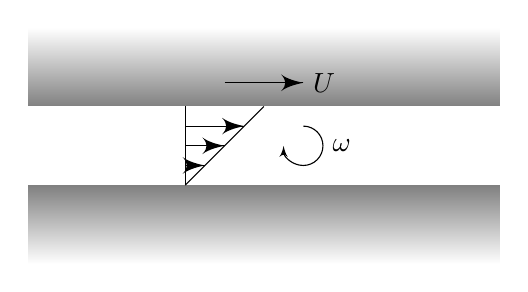
\begin{tikzpicture}
      \fill [gray, path fading=south] (0, 0) rectangle (6, -1);
      \fill [gray, path fading=north] (0, 1) rectangle (6, 2);
      \draw [->] (2.5, 1.3) -- +(1, 0) node [right] {$U$};

      \draw (2, 0) -- (2, 1);
      \draw (2, 0) -- (3, 1);

      \foreach \x in {0.25,0.5,0.75} {
        \draw [->] (2, \x) -- +(\x, 0);
      }
      \draw [-latex'] (3.5, 0.75) arc(90:-180:0.25);
      \node at (3.75, 0.5) [right] {$\omega$};
    \end{tikzpicture}
  \end{center}
  For the case of the Pouseuille flow, we have
  \[
    \boldsymbol\omega = \left(0, 0, \frac{G}{\mu}\left(y - \frac{h}{2}\right)\right).
  \]
\end{eg}
\begin{center}
  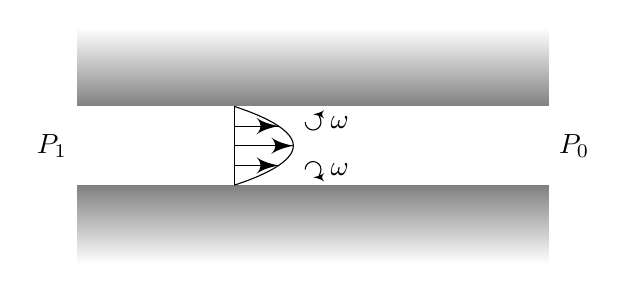
\begin{tikzpicture}
    \fill [gray, path fading=south] (0, 0) rectangle (6, -1);
    \fill [gray, path fading=north] (0, 1) rectangle (6, 2);

    \node [left] at (0, 0.5) {$P_1$};
    \node [right] at (6, 0.5) {$P_0$};

    \foreach \x in {0.25,0.5,0.75} {
      \pgfmathsetmacro\len{\x * (1 - \x)}
      \draw [->] (2, \x) -- +(3 * \len, 0);
    };
    \draw [rotate=270, yscale=-1, shift={(-3,-3)}] (2.5, 0.25) parabola (2, 1); % magic
    \draw [rotate=90, shift={(-2,-3)}] (2.5, 0.25) parabola (2, 1);
    \draw (2, 0) -- (2, 1);

    \draw [-latex'] (2.9, 0.2) arc(180:-90:0.1);
    \node at (3.1, 0.2) [right] {$\omega$};

    \draw [-latex'] (2.9, 0.8) arc(-180:90:0.1);
    \node at (3.1, 0.8) [right] {$\omega$};
  \end{tikzpicture}
\end{center}

\subsubsection{Surface stress}
Recall that $\tau_s$ is the tangential force per unit area exerted by the fluid on the surface, given by
\[
  \tau_s = \mu \frac{\partial u}{\partial \mathbf{n}},
\]
with $\mathbf{n}$ pointing into the fluid.

\begin{eg}
For the Couette flow, we have
\[
  \tau_s =
  \begin{cases}
    \mu \frac{U}{h} & y = 0\\
    -\mu \frac{U}{h} & y = h
  \end{cases}
\]
We see that at $y = 0$, the stress is positive, and pulls the surface forward. At $y = h$, it is negative, and the surface is pulled backwards.

For the Pouseuille flow, we have
\[
  \tau_s =
  \begin{cases}
    \frac{Gh}{2} & y = 0\\
    \frac{Gh}{2} & y = h\\
  \end{cases}
\]
Both surfaces are pulled forward, and this is independent of the viscosity. This makes sense since the force on the surface is given by the pressure gradient, which is independent of the fluid.
\end{eg}
\subsection{Gravity-driven flow down a slope}
\begin{center}
  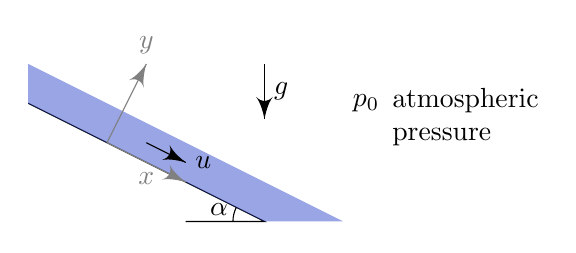
\begin{tikzpicture}
    \draw (0, 1.5) -- (3, 0) -- (2, 0);
    \fill [mblue, opacity=0.5] (0, 1.5) -- (3, 0) -- (4, 0) -- (0, 2) -- cycle;

    \draw [gray, ->] (1, 1) -- +(0.5, 1) node [above] {$y$};
    \draw [gray, ->] (1, 1) -- +(1, -0.5) node [below, pos=0.5] {$x$};
    \draw [->] (3, 2) -- +(0, -0.7) node [pos=0.5, right] {$g$};
    \draw [->] (1.5, 1) -- (2, 0.75) node [right] {$u$};
    \node [right] at (4, 1.5) {$p_0$};
    \node [right, align=left] at (4.5, 1.33) {atmospheric\\ pressure};
    \draw (2.6, 0) arc(180:153.4349:0.4);
    \node [left] at (2.66, 0.15) {$\alpha$};
  \end{tikzpicture}
\end{center}
Here there is just atmosphere above the fluid, and we assume the fluid flow is steady, ie. $u$ is merely a function of $y$. We further assume that the atmospheric pressure does not vary over the vertical extent of the flow. This is a very good approximation because $\rho_{\mathrm{air}} \ll \rho_{\mathrm{liq}}$.

Similarly, we assume $\mu_{\mathrm{air}} \ll \mu_{\mathrm{liq}}$. So the air exerts no significant tangential stress. This is known as a free surface.

We first solve the $y$ momentum equation. The force in the $y$ direction is $-g \rho \cos \alpha$. Hence the equation is
\[
  \frac{\partial p}{\partial y} = - gp \cos \alpha.
\]
Using the fact that $p = p_0$ at the top boundary, we get
\[
  p = p_0 - g\rho \cos \alpha (y - h).
\]
In particular, $p$ is independent of $x$. In the $x$ component, we get
\[
  \mu \frac{\partial^2 u}{\partial y^2} = g\rho \sin \alpha.
\]
The no slip condition gives $u = 0$ when $y = 0$. The other condition is that there is no stress at $y = h$. So we get $\frac{\partial u}{\partial y} = 0$ when $y = h$.

The solution is thus
\[
  u = \frac{gp\sin \alpha}{2 \mu} y(2h - y).
\]
This is a bit like the Poiseuille flow, with $\frac{gp \sin \alpha}{2\mu}$ as the pressure gradient. But instead of going to zero at $y = h$, we get to zero at $y = 2h$ instead. So this is half a Poiseuille flow. % diagram

It is an exercise for the reader to calculate the volume flux $q$.

% can insert profile
\subsection{Unsteady parallel viscous flow}
Consider fluid initially at rest in $y > 0$, resting on a flat surface.
\begin{center}
  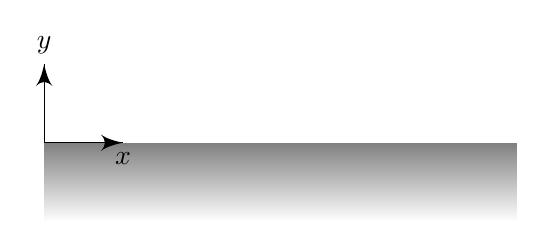
\begin{tikzpicture}
    \fill [gray, path fading=south] (0, 0) rectangle (6, -1);
    \draw [->] (0, 0) -- (0, 1) node [above] {$y$};
    \draw [->] (0, 0) -- (1 , 0) node [below] {$x$};
  \end{tikzpicture}
\end{center}
At time $t = 0$, the boundary $y = 0$ starts to move at constant speed $U$. There is no force and no pressure gradient.

We use the $x$-momentum equation to get
\[
  \frac{\partial u}{\partial t} = \nu \frac{\partial^2 u}{\partial y^2},
\]
where $\nu = \frac{\mu}{\rho}$. This is clearly the diffusion equation, with the diffusivity $\nu$. We can view this as the diffusion coefficient for motion/momentum/vorticity.
\begin{defi}[Kinematic viscosity]
  The \emph{kinematic viscosity} is
  \[
    \nu = \frac{\mu}{\rho}.
  \]
\end{defi}
The boundary conditions are $u = 0$ for $t = 0$ and $u \to 0$ as $y \to \infty$ for all $t$. The other boundary condition is obviously $u = U$ when $y = 0$, for $t > 0$.

You should have learnt how to solve this in, say, IB Methods. We will approach this differently here.
\subsubsection{Dimensional analysis}
We want to do some dimensional analysis. We are already provided with a velocity $U$. We let $T$ be our time scale. We would like to know how fast the movement of fluid propagates up the $y$ axis. We note that in this case, we don't really have an extrinsic length scale --- in the case where we have two boundaries, the distance between them is a natural length scale to compare with, but here the fluid is infinitely thick. So we need to come up with a characteristic intrinsic length scale somewhat arbitrarily. For example, at any time $T$, we can let $\delta$ be the amount of fluid that has reached a speed of at least $\frac{U}{10}$.

Instead of trying to figure out the dimensions of, say, $\nu$ and trying to match them, we just replace terms in the differential equation with these quantities of the right dimension, since we know our differential equation is dimensionally correct. So we obtain
\[
  \frac{U}{T} \sim \nu \frac{U}{\delta^2}.
\]
Since the $U$ cancels out, we get
\[
  \delta \sim \sqrt{\nu T}.
\]
We can figure out approximately how big this is. For water, we have $\nu_{\mathrm{water}} \approx \SI{10e-6}{\meter\squared\per\second}$. For air, we have $\nu_{\mathrm{air}} \approx \SI{10e-5}{\meter\squared\per\second}$. These are, in general, very tiny.
\end{document}
